% This is an included file. See the master file for more information.
%

\section{Execution Model}
\index{Execution Model}
\label{sec:ExecutionModel}

OCR is based on an asynchronous task model. The work of an OCR program
is defined in terms of a collection of tasks  organized
into a directed acyclic graph (DAG)\index{DAG}~\cite{TaSa11,Tasirlar11,Zuckerman:2011:UCP:2000417.2000424}.
Task execution is managed by the availability of data (the ``data
blocks'') and events; hence the reason the tasks are called ``Event
Driven Tasks'' or EDTs.

An OCR program executes on an abstract machine called the \emph{OCR
Platform}\index{OCR Platform}. The OCR platform is a resource that can carry out
computations. It consists of:
\begin{itemize}
\item A collection of network connected nodes where any two nodes can
communicate with each other.
\item Each node consists of one or more processing elements each of
which may have its own private memory\footnote{By ``private'' we mean a
memory region that is not accessible to other processing
elements.}.
\item Workers that run on the processing elements to execute enqueued EDTs.
\item A globally accessible shared name space of OCR objects each
denoted by a globally unique ID (GUID).
\end{itemize}
OCR is designed to be portable and scalable, hence, the OCR Platform
places minimal constraints on the physical hardware.


% TODO: Expand on "library mode" vs. "run alone"

The OCR program logically starts as a single EDT called \code{mainEDT()}.
In other words, the programmer does not provide a \code{main()} function.
The OCR runtime system creates the \code{main()} function on the programmer`s
behalf to set up the OCR environment and then calls the user provided
\code{mainEDT()}. The expected function prototype for the
\code{mainEDT()} is described in section~\ref{sec:mainEDT}.

The DAG corresponding to the executing program is constructed
dynamically and completes when the
\code{ocrShutdown()} or \code{ocrAbort()} function is called.
This rather simple model can handle a wide range of
design patterns including branch and bound, data flow, and divide and
conquer.
%
% TODO: Expression of SPMD algorithms in OCR

To understand the execution model of OCR, consider the discrete states and
transitions of an executing EDT as defined in figure~\ref{fig:EDTexec}. An
EDT is created and once its GUID is available for use in API
functions, the EDT is said to be \emph{Available}\index{EDT state,
  available}. At some point, the dependences are fully defined (all
pre-slots of the EDT are ``connected'') for the EDT and it becomes
\emph{Resolved}\index{EDT state, resolved}.
Note that the transition from \emph{Available} to \emph{Resolved} is
not called out as a named transition. This implies that it is not
generally possible for the system to set a distinct time-stamp
corresponding to when the transition occurred. In this case, the transition is un-named
because dependences may be added dynamically up until the
EDT \emph{Launch}\index{Launch} transition. At this point the
EDT is \emph{Runnable}\index{Runable}.

Once an EDT is runnable, it will execute at some point during the normal execution
of the OCR program. At some point all data blocks linked to an EDT
will be acquired and the EDT becomes \emph{Ready}\index{EDT state, ready}. The
EDT and any resources required to support its execution are then submitted to
\emph{workers}\index{Worker}~\cite{GBRS09} which execute the tasks on
the processing elements within the OCR platform. The workers and the
data-structures used to store tasks waiting to execute
(i.e.\ work-pools) are a low level implementation detail not defined by
the OCR specification. When reasoning about locality and load
balancing, programmers may need to explicitly reason about the
behavior of the workers~\cite{Chatterjee13}, but they do not hold
persistent state visible to an OCR program and are logically opaque to
OCR constructs. The scheduler inside the implementation of OCR
will then schedule the EDT for execution and the EDT
\emph{Starts}\index{EDT state, start} to execute and
becomes a \emph{Running}\index{EDT state, running} EDT.

% TODO: Add extra transitions in the graph from certain states to destroyed state,
% for when the user cancels the EDT

\begin{figure*}
\centering
 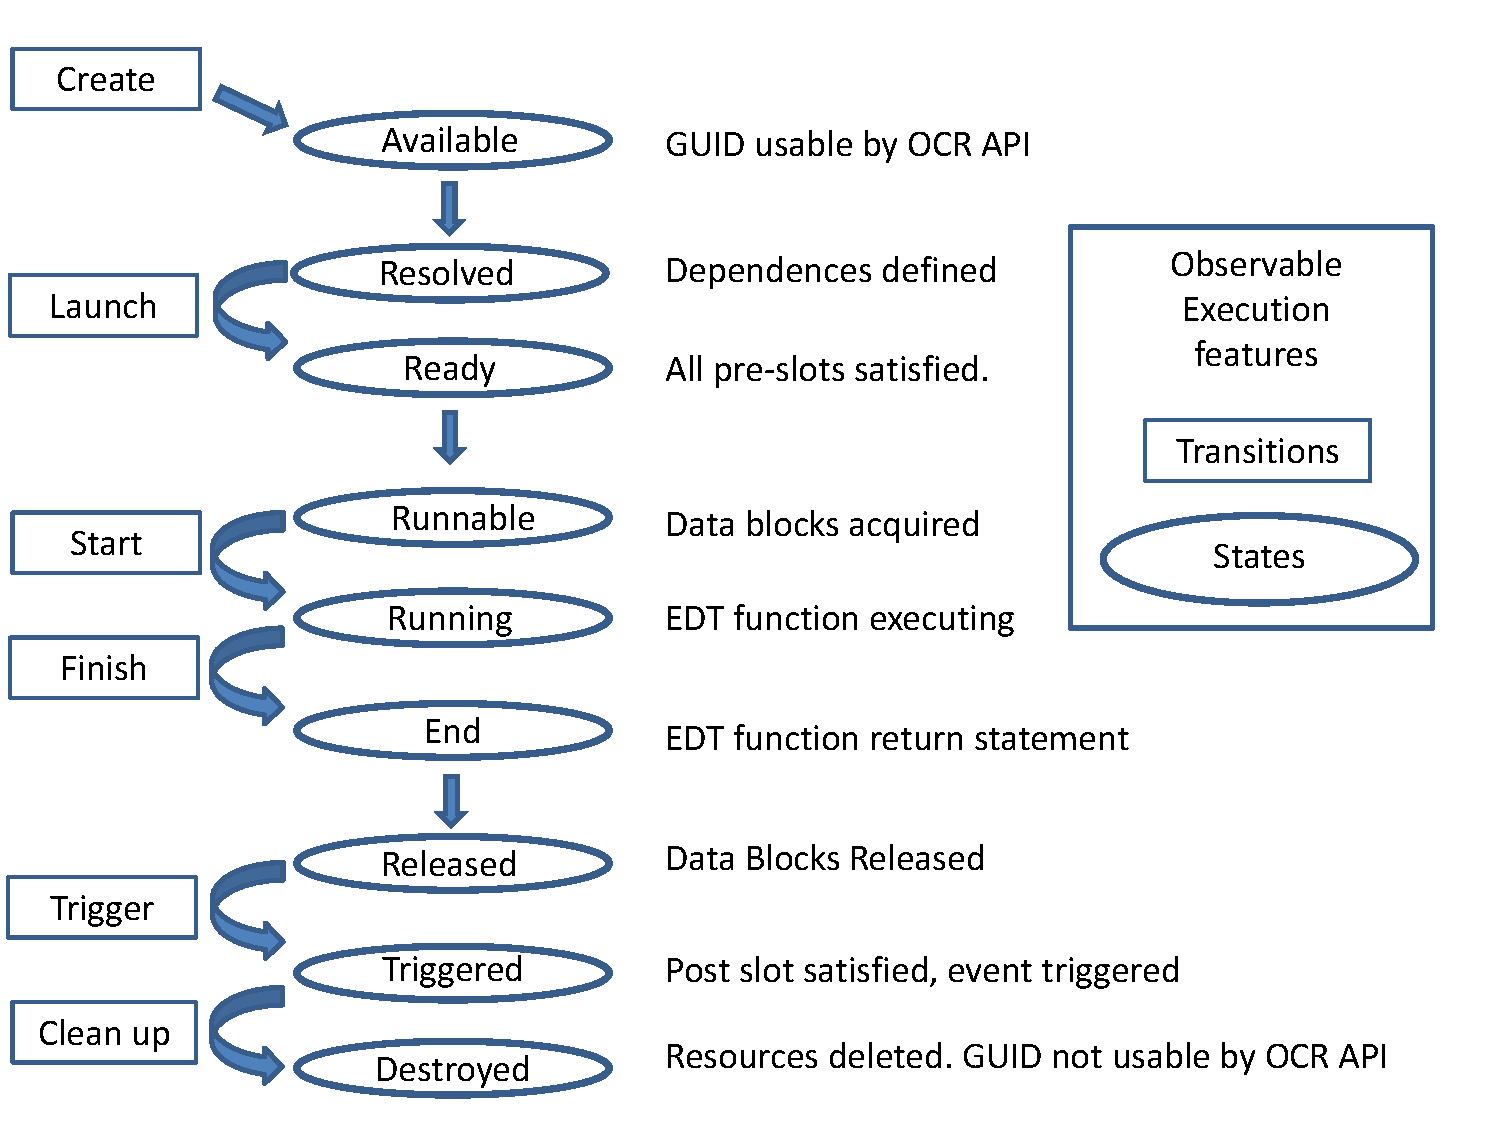
\includegraphics[width=0.9\textwidth]{EDT_exec}
\caption{Observable execution features.}
\label{fig:EDTexec}
\end{figure*}

Normal EDT execution continues until the EDT function returns. The EDT undergoes
a \emph{Finish}\index{EDT transition, finish} transition and the EDT is in
the \emph{End}\index{EDT state, end} state. At some point the EDT will
release the data blocks associated with the EDTs execution and the
EDT enters the \emph{Released}\index{EDT state, released} state.
At this point, any changes made to data blocks will
be available for use by other OCR objects. Later the EDT will
mark its post-slot as satisfied to \emph{Trigger}\index{Trigger} the event
associated with the EDT; thereby becoming a \emph{Triggered} EDT. At
some later point the
system will \emph{Clean-up}\index{EDT transition, clean-up} resources
used by the EDT (including its GUID) and the EDT is destroyed.

Since an EDT is non-blocking, once it
becomes \emph{Runnable} it will run on the OCR platform at some point in the
future. During its run:
\begin{itemize}
\item The EDT can only access data blocks that have been passed in
through its pre-slots as well as any data blocks that the EDT creates
internally. This means that before an EDT starts, the OCR runtime
knows all the data blocks that will be accessed (minus the ones
created within the EDT).

\item The EDT can call into the runtime to create and destroy data
blocks, EDTs and events.

\item The EDT can create \emph{links} between the various OCR
software constructs, termed \emph{dependences}. This is
accomplished through the \code{ocrAddDependence()} function of the OCR
API. The following types of dependences can be created:
\begin{itemize}
\item \emph{Event to Event}: The destination event’s pre-slot is chained
directly to the source event’s post-slot.
For all events but the latch event, this means that the triggering of
the source event will trigger the destination event.

\item \emph{Event to EDT}: One of the destination EDT’s pre-slot is chained
directly to the source event’s post-slot. When the source event is
triggered, this will satisfy the EDT’s pre-slot. If a data-block was
associated with the triggering of the source event, that data-block
will be made available to the EDT in the dependence array in the
position of the pre-slot. This is a “control + data” dependence. In
the other case, no data-block will be made available and the
dependence is akin to a pure control dependence.

\item \emph{Data Block to Event}: Adding a dependence between a data-block and an
event is equivalent to satisfying the event with the data-block.

\item \emph{Data Block to EDT}: Directly adding a dependence between a data-block and
an EDT (a pure data-dependence) immediately satisfies the EDT’s
pre-slot and makes the data-block available to the EDT in the
dependence array in the position of the pre-slot.
\end{itemize}

\item The EDT cannot perform any synchronization operations that would
cause it to block inside the body of the task (i.e.\ the EDT must be
non-blocking). The only mechanism for synchronization within OCR is
through the events that link OCR objects, which are explicit to the
runtime.
\end{itemize}

% TODO: Add clarity to the following paragraph on when a programmer
% calls ocrShutdown to terminate even when a few other EDTs haven't
% completed execution, how much is being presumed.

A computation is complete when an EDT terminates the program
(e.g.\ with a call to \code{ocrShutdown()}). Typically, the EDT that
terminates the program is the last EDT in the program DAG, and the
programmer has assured that all other EDTs in the DAG have completed
execution before the function to terminate the program is called.

Since the OCR runtime creates the \code{main()}
function, the programmer does not need to manage the low level
details of initializing and cleanly shutting down OCR.

With both data and tasks conceptually decoupled from their realization
on a computer system, OCR has the flexibility to relocate tasks and data
to respond to failures in the system, achieve a better balance of load
among the processing elements of the computer, or to optimize memory
and energy consumption~\cite{GZCS10,Guo10,CTBCCGYS13,SbBS14}.
This requires that the state of an OCR program can be defined
strictly in terms of which tasks have completed their execution
and the history of updates to data blocks. By saving a log of updates to Data blocks
relative to the tasks that have completed execution, the system can recover
the state of a computation should components of the system fail. This requires,
however, that EDTs execute with transactional semantics.

% This is the end of ch1-exec.tex of the OCR specification.
